\documentclass{beamer}
%\usepackage{beamerthemebars}


%%% EU logo
% small version for upper right corner of normal pages
\pgfdeclareimage[width=12.8cm]{university-logo}{JRC_header}
\logo{\pgfuseimage{university-logo}}
\pgfdeclareimage[height=5.5mm]{footimage}{JRC_footer}
\newcommand{\titleimage}[1]{\pgfdeclareimage[width=0.5\textwidth]{title-image}{#1}}
%\newcommand{\footimage}{\pgfdeclareimage[width=0.5\textwidth]{title-image}{#1}}
\titlegraphic{\pgfuseimage{title-image}}
%%% end EU logo

% NOTE: 1cm = 0.393 in = 28.346 pt;    1 pt = 1/72 in = 0.0352 cm
\setbeamersize{text margin right=3.5mm, text margin left=7.5mm}  % text margin

% colors to be used
\definecolor{text-grey}{rgb}{0.45, 0.45, 0.45} % grey text on white background
\definecolor{bg-grey}{rgb}{0.66, 0.65, 0.60} % grey background (for white text)
\definecolor{eu-blue}{RGB}{55, 172, 222} % blue text
\definecolor{drk-blue}{RGB}{0, 51, 102} % blue text
\definecolor{fu-blue}{RGB}{0, 51, 102} % blue text
\definecolor{fu-green}{RGB}{153, 204, 0} % green text
\definecolor{fu-red}{RGB}{204, 0, 0} % red text (used by \alert)

% switch off the sidebars
\setbeamersize{sidebar width left=0cm, sidebar width right=0mm}
\setbeamertemplate{sidebar right}{}
\setbeamertemplate{sidebar left}{}
\setbeamertemplate{navigation symbols}{}%remove navigation symbols

% frame title
\setbeamertemplate{frametitle}{%
    \vskip-5pt \color{drk-blue}\Large%
    \begin{minipage}[b][23pt]{\textwidth}%
    \flushleft \textbf{\insertframetitle}%
    \end{minipage}%
}

%%% title page
\setbeamertemplate{title page}{

% set the title
\parbox[top][2.8cm][c]{\textwidth}{\begin{center} \color{drk-blue}\LARGE \textbf{\inserttitle}  \\ \vspace{10pt} \small \insertsubtitle \end{center}}

% title image of the presentation
\begin{minipage}{0.5\textwidth}
\flushleft
%\hspace{-7.5mm}
\inserttitlegraphic
\end{minipage}
% Author info
\hspace{0.5cm}
\begin{minipage}{0.4\textwidth}
{\flushleft \color{black} \textbf{\insertauthor} \\ \insertinstitute }
\end{minipage}
}
%%% end title page

%%% colors
\usecolortheme{lily}
\setbeamercolor*{normal text}{fg=drk-blue, bg=white}
\setbeamercolor*{alerted text}{fg=fu-red}
\setbeamercolor*{example text}{fg=fu-green}
\setbeamercolor*{structure}{fg=fu-blue}

\setbeamercolor*{block title}{fg=white,bg=black!50}
\setbeamercolor*{block title alerted}{fg=white,bg=black!50}
\setbeamercolor*{block title example}{fg=white,bg=black!50}

\setbeamercolor*{block body}{bg=black!10}
\setbeamercolor*{block body alerted}{bg=black!10}
\setbeamercolor*{block body example}{bg=black!10}

\setbeamercolor{item}{fg=eu-blue}
%%% end colors

\setbeamertemplate{itemize items}[circle] % if you want a ball
\setbeamertemplate{itemize subitem}[circle] % if you wnat a circle
\setbeamertemplate{itemize subsubitem}[cirlce] % if you want a triangle

%%% headline
\setbeamertemplate{headline}{
\insertlogo % logo on the right
%\begin{center}
%\colorbox{eu-blue}{
% \begin{minipage}[t]{.8\textwidth} \color{eu-blue} text \vspace{25pt} %\end{minipage}}
%\begin{minipage}[c]{0.0\textwidth}
%\hspace{-10mm} hi
%\end{minipage}
%\end{center}
}
%%% end headline

%%% footline
\newcommand{\footlinetext}{\insertdate}
\setbeamertemplate{footline}{
\begin{minipage}{58mm}
 \color{drk-blue} \hspace{7.5mm} \footlinetext
\end{minipage}
\hspace{0.1mm} 
\begin{minipage}{8.5mm}
 \pgfuseimage{footimage}
\end{minipage}
\hspace{0.1mm}
\begin{minipage}{50mm}
 \color{drk-blue} 
 %\raisebox{-1pt}{\usebeamertemplate***{navigation symbols}}
 \flushright \insertframenumber
\end{minipage}

}
%%% end footline
    % THIS is the line that includes the EU template!
\usepackage{arev,t1enc}
\usepackage{amsmath}

\usepackage[T1]{fontenc}
\fontfamily{verdana}\selectfont

\titleimage{koter} % pdf or png
\title{The Costs of Ignoring Stock Structure}
\subtitle{How VMS and logbook data might be used to compliment surveys}
\author[CP Millar]{Colin Millar}
\institute[JRC]{European Commission\\ Joint Research Center}
\date[Sketch 2012]{30 March 2012}
\subject{Fisheries Management}

\newcommand{\ee}{\stackrel{e}{=}}
\usepackage{Sweave}


\begin{document}
\setkeys{Gin}{width=1.1\textwidth}


\begin{frame}
\titlepage
\end{frame}

\section{Introduction}
\label{sec:introduction}

\begin{frame}
\begin{center}
\LARGE \textbf{$\text{Catch} = q \times \text{Abundance}$}
\end{center}
\end{frame}

\begin{frame}{$\text{Catch} = q \times \text{Abundance}$}
The problem with fishers is that they do not 'sample' \textbf{uniformly}\\
\begin{minipage}{0.4\textwidth}
  \begin{flushleft}
    A uniform distribution
    \begin{align*}
      \text{Index} = \frac{N}{n} \sum_{i=1}^n catch_i    
    \end{align*}
    $n =$ no. of samples \\
    $N =$ no. of sampling units
  \end{flushleft}
\end{minipage}
\hspace{0.5cm}
\begin{minipage}{0.4\textwidth}
  \begin{figure}
    \centering
    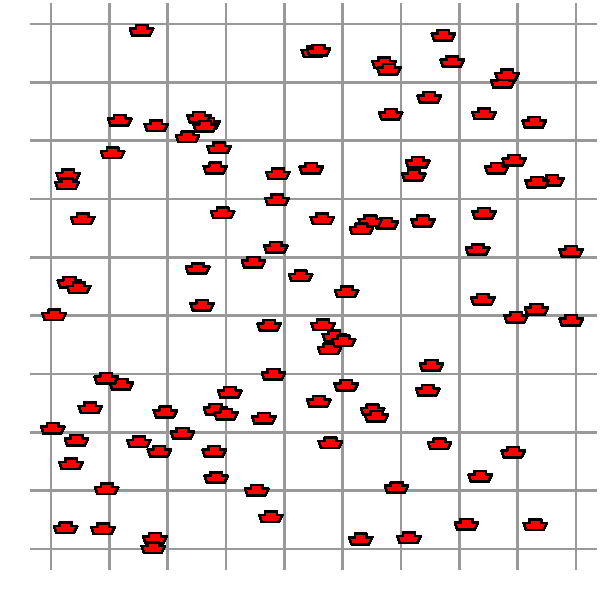
\includegraphics[width=5.5cm]{fig1}
  \end{figure}
\end{minipage}

\end{frame}

\begin{frame}{$\text{Catch} = q \times \text{Abundance}$}
Fishing tends to be a focused activity\\
\begin{minipage}{0.4\textwidth}
  \begin{flushleft}
    \begin{align*}
      \text{Index} \neq \frac{N}{n} \sum_{i=1}^n catch_i    
    \end{align*}
    $n =$ no. of samples \\
    $N =$ no. of sampling units
  \end{flushleft}
\end{minipage}
\hspace{0.5cm}
\begin{minipage}{0.4\textwidth}
  \begin{figure}
    \centering
    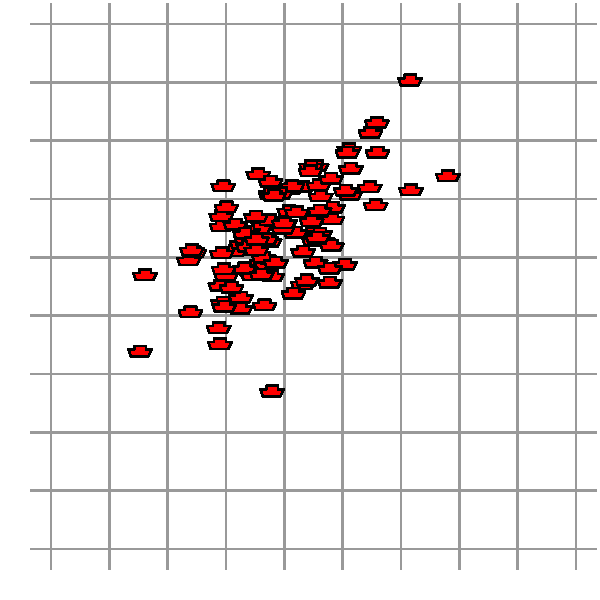
\includegraphics[width=5.5cm]{fig2}
  \end{figure}
\end{minipage}
\end{frame}


\begin{frame}{$\text{Catch} = q \times \text{Abundance}$}
So there is an unequal probability of sampling\\
\begin{minipage}{0.4\textwidth}
  \begin{flushleft}
    Unequal probability sampling \\
    Hansen-Hurwitz estimator\\    
    \begin{align*}
      \text{Index} = \frac{1}{n} \sum_{i=1}^n \frac{catch_i}{p_i}  
    \end{align*}
    $n =$ no. of samples \\
    $p_i =$ probability of sampling
  \end{flushleft}
\end{minipage}
\hspace{0.5cm}
\begin{minipage}{0.4\textwidth}
  \begin{figure}
    \centering
    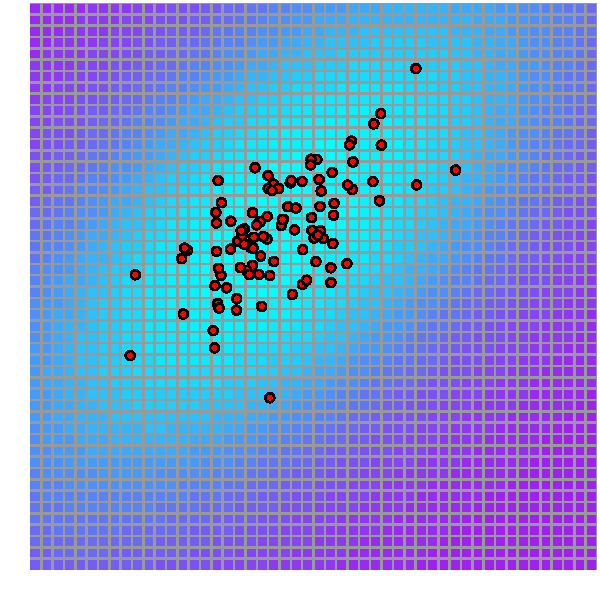
\includegraphics[width=5.5cm]{fig3}
  \end{figure}
\end{minipage}
\end{frame}

\begin{frame}{$\text{Catch} = q \times \text{Abundance}$ (in \alert{fished} area)}
There are also regions that are never sampled\\
\begin{minipage}{0.4\textwidth}
  \begin{flushright}
    A non uniform distribution with regions of \alert{\textbf{zero}} sampling probability \\
    \begin{align*}
      \text{Index}_\text{fished population} & \\
       = \frac{1}{n} &\sum_{i=1}^n \frac{catch_i}{p_i}  
    \end{align*}  
  \end{flushright}
\end{minipage}
\hspace{0.5cm}
\begin{minipage}{0.4\textwidth}
  \begin{figure}
    \centering
    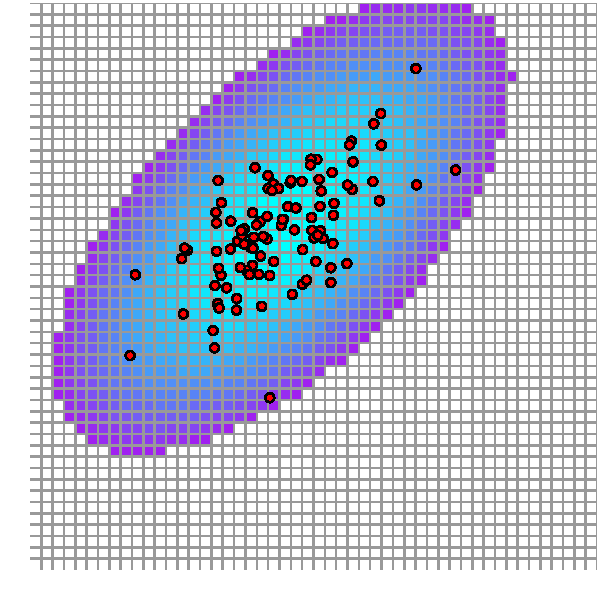
\includegraphics[width=5.5cm]{fig4}
  \end{figure}
\end{minipage}
\end{frame}


\begin{frame}{$\text{Catch} = q \times \text{Abundance}$ (in \alert{fished} area)}
What is the probability of sampling?\\
\begin{minipage}{0.4\textwidth}
  \begin{flushright}
    Use the spatial location of fishing pings to estimate the probability of sampling\\
    \begin{align*}
      \text{Index}_\text{fished population} & \\
       = \frac{1}{n} &\sum_{i=1}^n \frac{catch_i}{\hat{p}_i}  
    \end{align*}  
  \end{flushright}
\end{minipage}
\hspace{0.5cm}
\begin{minipage}{0.4\textwidth}
  \begin{figure}
    \centering
    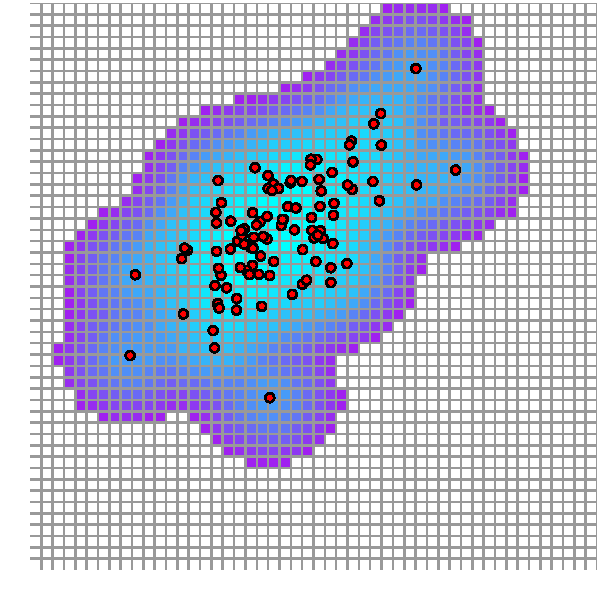
\includegraphics[width=5.5cm]{fig5}
  \end{figure}
\end{minipage}
\end{frame}

\begin{frame}{Comparing with Survey Data}
We can also estimate the surface of $q \times \text{Abundance}$
\begin{minipage}{0.4\textwidth}
  \begin{flushright}
    Use the spatial location of fishing pings and catch observations to estimate a \alert{\textbf{smooth}} density surface
    \begin{align*}
      E[catch_i] = D_{loc(i)}  
    \end{align*}
    where $D$ has spatial structure    
  \end{flushright}
\end{minipage}
\hspace{0.5cm}
\begin{minipage}{0.4\textwidth}
  \begin{figure}
    \centering
    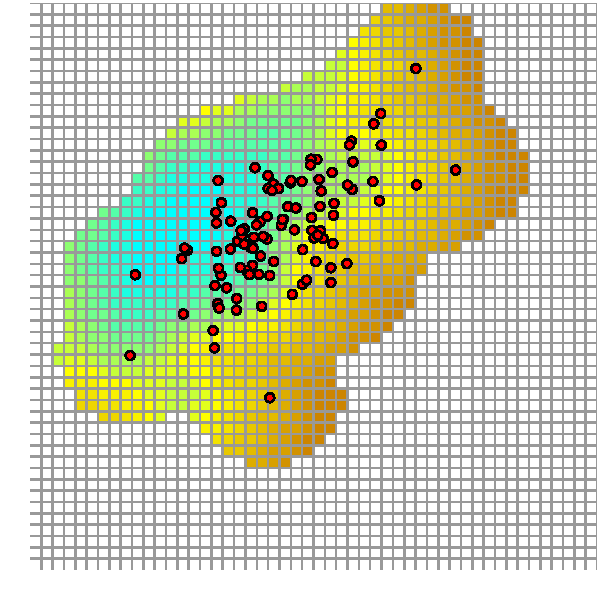
\includegraphics[width=5.5cm]{fig6}
  \end{figure}
\end{minipage}
\end{frame}

\begin{frame}{Filling in the gaps}
To combine we need the ratio in catchabilities\\
\begin{minipage}{0.4\textwidth}
  \begin{flushleft}
    \begin{align*}
      E[catch_i] &= D_{loc(i)} \\
      E[survey_j] &= r \times D_{loc(j)}  
    \end{align*}
    where
    \begin{align*}
      r = \frac{q_{surv}}{q}  
    \end{align*}    
  \end{flushleft}
\end{minipage}
\hspace{0.5cm}
\begin{minipage}{0.4\textwidth}
  \begin{figure}
    \centering
    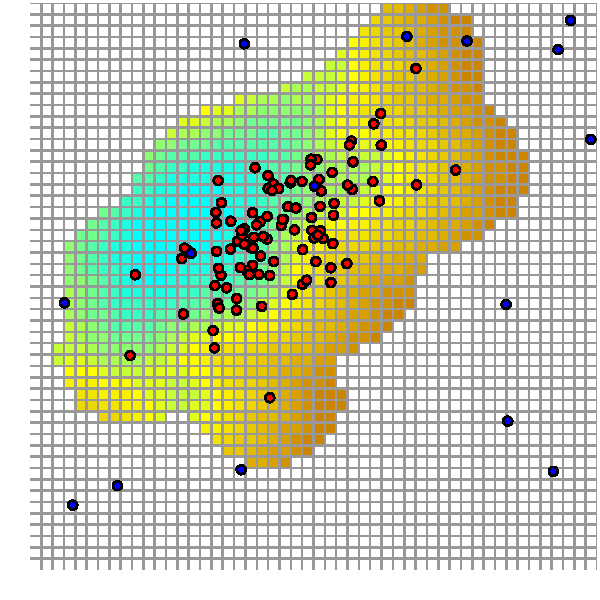
\includegraphics[width=5.5cm]{fig7}
  \end{figure}
\end{minipage}
\end{frame}

\begin{frame}{Filling in the gaps}
Combining survey and catch data\\
\begin{minipage}{0.4\textwidth}
  \begin{flushleft}
    \begin{align*}
      \frac{1}{n} \sum_{i=1}^n \frac{catch_i}{\hat{p}_i} + 
      r \frac{N_s}{n_s} \sum_{i=1}^{n_s} survey_i
    \end{align*}
    \vspace{6pt}
    $n_s =$ no. of survey samples \\
    $N_s =$ no. of 'unfished' units \\
    $r =$ the catchability ratio
  \end{flushleft}
\end{minipage}
\hspace{0.5cm}
\begin{minipage}{0.4\textwidth}
  \begin{figure}
    \centering
    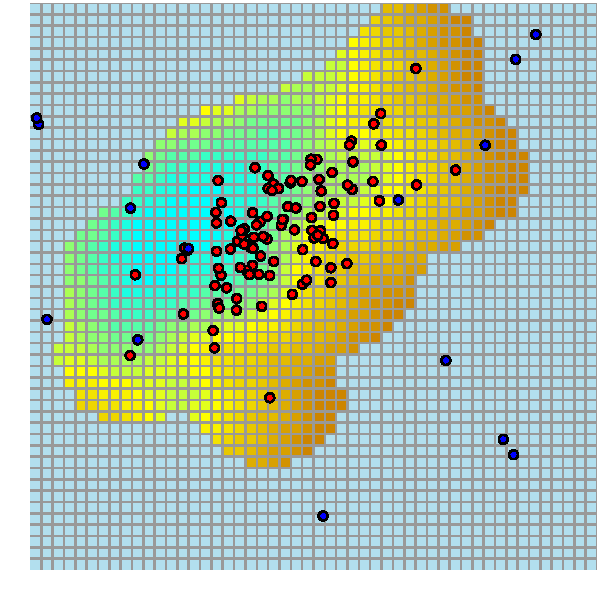
\includegraphics[width=5.5cm]{fig8}
  \end{figure}
\end{minipage}
\end{frame}


\begin{frame}{VMS - Vessel Monitoring System}
  Reports the position of a vessel every 2 hours \\
  Also reports speed and vessel ID
  
\end{frame}


\end{document}
